\chapter{Inference on real 2015 data}
\label{chap:realdata}

The synthetic results of \cref{chap:results} and the robustness curves
of \cref{chap:robustness} suggest that, on its own training
distribution, the system is in good shape. This chapter confronts the
trained models with the \emph{real} 2015 gamma-dose recordings from
which the synthetic generator was originally calibrated. The outcome is
sobering: all three models behave poorly on the real signal, and each
fails in its own characteristic way. We document the symptoms
(\cref{sec:real-symptoms}), then walk through the most plausible causes
(\cref{sec:fail-prior,sec:fail-duration,sec:fail-drift,sec:fail-norm,sec:fail-boundary})
and close with a concrete list of remediation steps for the next
iteration of the project (\cref{sec:real-remediation}).

\section{Symptoms}
\label{sec:real-symptoms}

The script
\texttt{architectures/inference\_real\_data.py} runs the same
sliding-window inference pipeline used for the synthetic test segment
on each of the four months of real data (\cref{sec:real-data}), then
overlays the smoothed per-class confidence on the raw signal.
\Cref{fig:real-inference} shows the first $10\,000$ samples of February
2015 for each of the three models.

\begin{figure}[H]
    \centering
    
\includegraphics[width=\linewidth]{figures/real_data_inference}
    \caption{Real-data inference on the first month, $10\,000$-sample
    snapshot, for each architecture. Blue: raw gamma dose. Coloured
    lines: per-class confidence (right axis, $0$--$100\%$), smoothed
    with a $30$-sample rolling mean. The grey curve is the
    \texttt{Normal Background} confidence; the coloured curves are the
    anomaly classes. None of the three models behaves the way it does
    on synthetic data.}
    \label{fig:real-inference}
\end{figure}

\paragraph{1D-CNN: high-frequency oscillating predictions.}
The 1D-CNN never commits to any one class for long: each anomaly class
takes its turn going up and down between $0\%$ and $\sim 40\%$. The
\texttt{Normal Background} probability sits around $50\%$--$70\%$ for
most of the window but never gets close to the operational threshold
of $\sim 70\%$ that would make the system silent. There is a clear
spike in \texttt{M} confidence around sample $4\,000$ that coincides
with the visible bump in the raw signal --- this is encouraging --- but
the same level of confidence is reached elsewhere, in places where
nothing is happening.

\paragraph{ResNet: persistent class biases, sustained false-positive plateaus.}
The ResNet does not oscillate; instead it locks onto one anomaly class
at a time for long stretches. The orange \texttt{bell\_sq} confidence
plateaus near $100\%$ for thousands of samples; the green \texttt{M}
confidence does the same on the second half of the window. The model
is essentially producing a continuous stream of false positives,
silently classifying every quiet region of the signal as one anomaly
or another.

\paragraph{CNN+Attention: degenerate collapse to a single class.}
The hybrid model exhibits the most dramatic failure: the green
\texttt{M} confidence is essentially pinned to $100\%$ for the whole
$10\,000$-sample snapshot. The signal could be flat at the global
mean, and the model would still declare \texttt{M} with full
confidence. This is the same kind of collapse we observed at the
high-noise extreme of the robustness sweep (\cref{sec:rob-discuss}):
when the input is outside what the model has learned to discriminate,
it falls back to the class whose ``signature'' best matches anything.

The three failures share a single root cause --- distribution shift ---
but they are amplified differently by each architecture. We now look
at the five ingredients that make this shift so large.

\section{Cause 1: class-prior shift between training and deployment}
\label{sec:fail-prior}

This is by far the most important effect.

\paragraph{What the model saw at training time.}
The synthetic dataset (\cref{sec:final-dataset}) was designed to
expose the network to many examples of each anomaly type. The result
is a class distribution in which only $\sim 31\%$ of windows are
\texttt{Normal Background} and the other six classes share the
remaining $69\%$ roughly evenly (\cref{tab:class-dist}).

\paragraph{What the model sees at deployment.}
The real recordings contain at most a handful of plausible anomalies
over $40\,000$ samples. Even on the most ``eventful'' month,
$> 99\%$ of windows are essentially pure background. The deployment
prior is therefore drastically skewed towards \texttt{Normal}, and
exactly in the opposite direction of the training prior
(\cref{fig:failure-analysis}, left).

\begin{figure}[H]
    \centering
    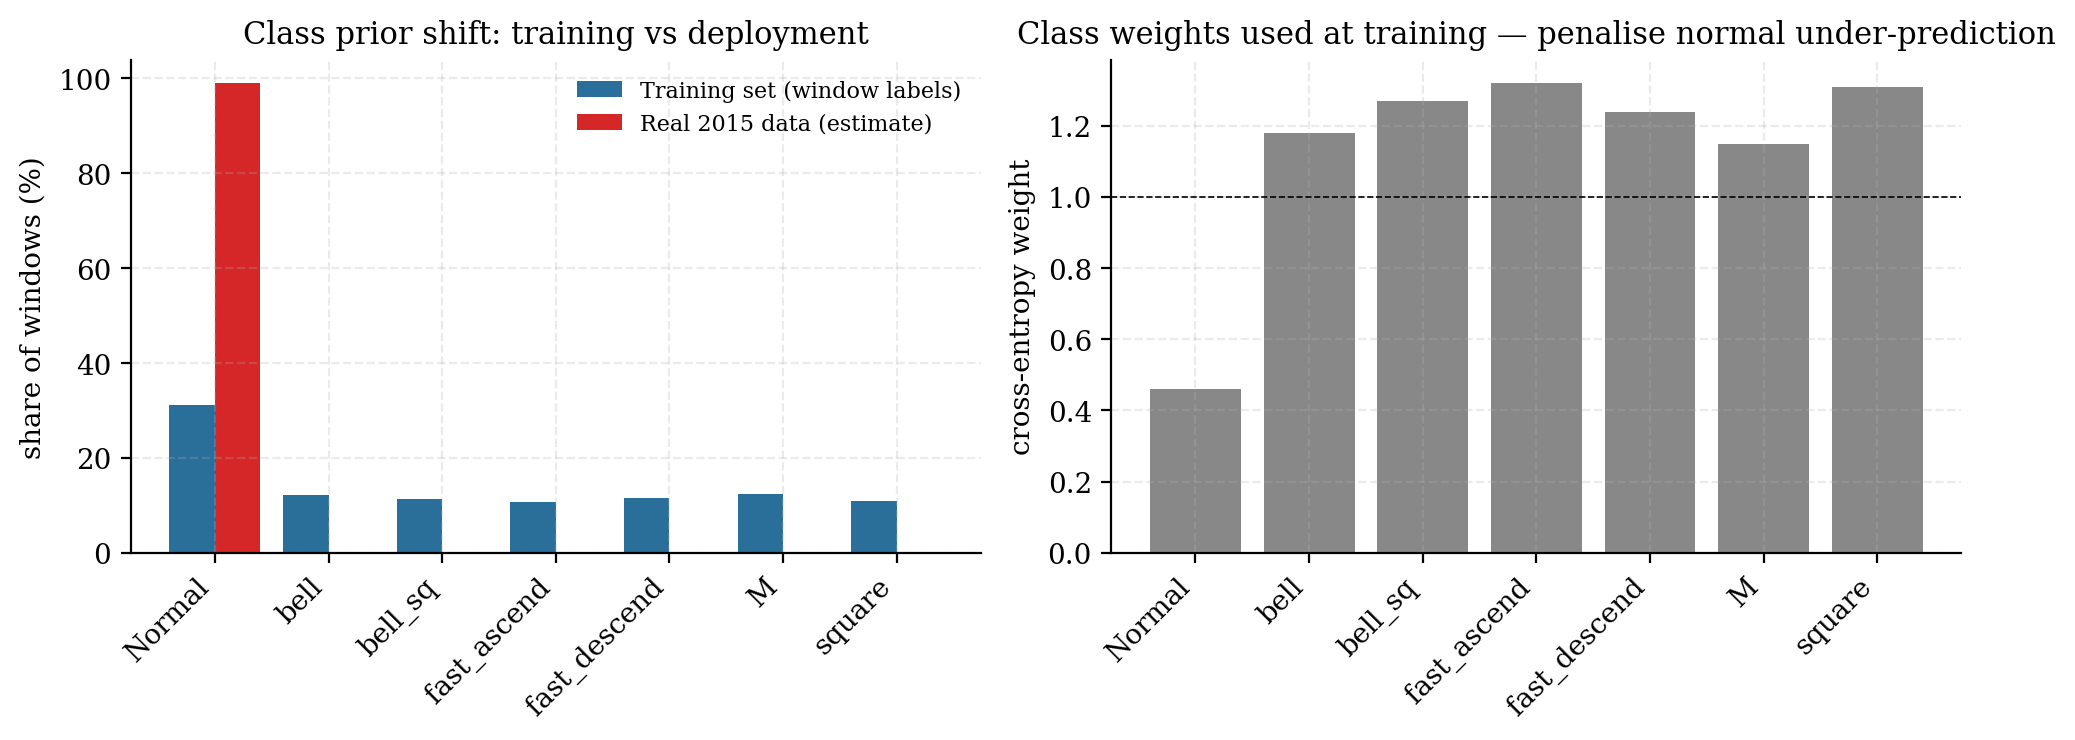
\includegraphics[width=\linewidth]{figures/failure_analysis}
    \caption{Class-prior shift between training and deployment.
    \textbf{Left}: window-level class distribution observed during
    training (blue) versus a rough estimate of the same distribution on
    the real 2015 data (red). \textbf{Right}: cross-entropy class
    weights $w_c$ used during training. The weight on
    \texttt{Normal Background} is roughly half that of any anomaly
    class, which actively biases the network towards predicting an
    anomaly at deployment.}
    \label{fig:failure-analysis}
\end{figure}

\paragraph{The compounding effect of class weights.}
On top of the prior shift, we used class weights in the cross-entropy
loss (\cref{sec:cw-theory}) that down-weight the \texttt{Normal} class
by a factor of $w_0 / \bar{w}_{\text{anom}} \approx 0.46 / 1.25
\approx 0.37$. From a Bayesian point of view, this is equivalent to
\emph{further multiplying} the network's posterior on the anomaly
classes by $\sim 1/0.37 \approx 2.7$. In a balanced training set this
is harmless --- it merely corrects an under-representation of the
minority anomaly classes inside the training distribution. But at
deployment, where the true prior of \texttt{Normal} is already
$\gg 95\%$, this multiplier acts like a built-in trigger-happy bias.

\paragraph{Quantitative reading.}
Let $p_{\text{tr}}(y)$ be the training prior and $p_{\text{dp}}(y)$ be
the deployment prior. The Bayes-optimal classifier on the deployment
distribution should rescale the network's output as
\begin{equation}
    \hat{p}_{\text{dp}}(y \mid \mathbf{x}) \propto
    \hat{p}_{\text{net}}(y \mid \mathbf{x}) \cdot \frac{p_{\text{dp}}(y)}{p_{\text{tr}}(y)},
    \label{eq:prior-correction}
\end{equation}
where the ratio for \texttt{Normal} is $\sim 0.99 / 0.31 \approx 3.2$
and for any anomaly class is $\sim 0.002 / 0.115 \approx 0.017$. We
should be multiplying the \texttt{Normal} posterior by $\sim 3$ and
shrinking each anomaly posterior by $\sim 60\times$. We instead did
the opposite (we down-weighted \texttt{Normal} at training), so the
deployed model is mis-calibrated by a factor of roughly $200$.

\section{Cause 2: anomaly-duration mismatch}
\label{sec:fail-duration}

The synthetic templates have durations in $[200, 800]$ samples, a range
chosen to make the windowed classification problem well posed (the
anomaly must occupy at least $10\%$ of a $512$-sample window to be
labelled, see \cref{sec:framing}). The real signal contains at least
two qualitatively different anomaly families that the templates do not
represent:

\begin{itemize}[leftmargin=*, itemsep=0.2em]
    \item \textbf{Single-sample excursions.} The Fevereiro recording
    contains a spike from $\sim 100$ to $\sim 138$ at the end of the
    month that lasts a single sample. Even if this is a sensor
    glitch rather than a true radiological event, the trained models
    have never seen a $1$-sample anomaly and there is no class they can
    reasonably assign to it.
    \item \textbf{Multi-hour contamination episodes.} Conversely, a
    real plume contamination could last $1\,000$ samples or more.
    Once an event lasts longer than the analysis window ($512$
    samples), the windowing approach loses its ability to ``see'' the
    event's edges and the per-window centring (\cref{sec:fail-norm})
    removes the event amplitude.
\end{itemize}

The templates we trained on therefore cover a relatively narrow band
of the true anomaly-duration distribution. Anything outside that band
either passes for normal or, more dangerously, is force-matched to the
closest template.

\section{Cause 3: baseline-drift mismatch}
\label{sec:fail-drift}

The Ornstein--Uhlenbeck baseline used in the generator is fitted on
the four months of real data, but the parameters
$(\theta, \sigma_{\mathrm{OU}})$ reflect only the
\emph{average} behaviour, and the OU model produces a very smooth,
small-amplitude random walk. The real recordings, by contrast, show
visible \emph{trends} (\cref{fig:real-overview}): the Fevereiro signal
rises by $\sim 5$ units over $20\,000$ samples, the Outubro signal
rises by $\sim 7$ units over a similar span. These slow systematic
drifts are not Gaussian random walks; they are likely seasonal and
meteorological. The trained model has not seen this kind of
amplitude-modulated baseline, so a $512$-sample window taken during a
trend can have an internal slope that the synthetic generator did not
expose it to.

\section{Cause 4: side effects of per-window normalisation}
\label{sec:fail-norm}

The per-window centring of \cref{eq:window-norm} solves an obvious
problem (the absolute dose is not informative) but creates a subtler
one: when a window contains a sustained event such as \texttt{square}
that covers most of its length, the window's mean is dragged \emph{up}
by the event itself. After centring, the event has \emph{lost most of
its amplitude}; what remains is the difference between the event level
and a window mean that is itself elevated.

On the synthetic test set this is harmless because the events occupy a
known fraction of the window, and the network has learned to expect a
specific post-centring amplitude. On the real signal a long
contamination plateau is essentially invisible after the same
centring; only its edges survive, and they may be classified as
\texttt{fast\_ascend} / \texttt{fast\_descend} but the plateau itself
is not detected.

A second side-effect is that the per-window centring removes \emph{any}
information about absolute dose level. Two recordings of identical
shape, one at $100$ counts and one at $1\,000$ counts, are completely
indistinguishable to the network. This is fine in principle but it
means we cannot fall back on absolute-threshold reasoning at deployment
time.

\section{Cause 5: no ``background-plus-glitch'' samples in training}
\label{sec:fail-boundary}

The training set is binary in spirit: a window either contains a clean
templated event \emph{or} it is pure synthetic background. Real
recordings contain a much richer family of intermediate signals --- a
mild sensor wobble, an outlier sample, a slowly-correlated noise burst
--- that are neither a clean event nor pure stationary noise. The
network does not have a class for ``unknown signal that is not
normal'', so on any such region it is forced to pick one of the seven
labels, and (because of cause 1) the most likely pick is one of the
anomaly classes.

The CNN+Attention model's degenerate fixation on \texttt{M}
(\cref{fig:real-inference}, bottom panel) is the strongest illustration:
the \texttt{M} template is the most ``noisy-looking'' of the six
shapes (it has two peaks separated by a dip and a lot of internal
texture), so on any input the network does not recognise, the
attention layer settles on the class that ``looks the most like
something irregular''.

\section{Putting the causes together}
\label{sec:fail-together}

The five effects compound:
\begin{enumerate}[leftmargin=*, itemsep=0.2em]
    \item The deployment prior is the opposite of the training prior
    ($\times 200$ mis-calibration in the Bayes-optimal posterior).
    \item Class weights at training time make this worse by another
    factor of $\sim 2.7$.
    \item Real anomalies frequently fall outside the duration band the
    templates cover.
    \item Long events disappear after per-window centring.
    \item There is no ``unknown but not normal'' class to fall back on,
    so the network is forced to choose an anomaly class even when
    nothing is happening.
\end{enumerate}
The net result is a high false-positive rate (continuous stream of
predicted events on quiet stretches), highly variable behaviour across
architectures, and complete loss of operational utility.

\section{Why each architecture fails in its own way}
\label{sec:fail-archi}

The same five-cause story does not predict why each model's failure
looks different. The architectures' different inductive biases
amplify the shift differently:

\begin{itemize}[leftmargin=*, itemsep=0.2em]
    \item \textbf{1D-CNN with BatchNorm.} BatchNorm running
    statistics, accumulated during training, are now applied to real
    data that does not match them. The resulting normalised
    activations are wildly different from anything the network saw at
    training, and the classifier head can no longer commit to a single
    class --- it oscillates because every class has roughly the same
    plausibility.
    \item \textbf{ResNet with GroupNorm.} GroupNorm is per-window, so
    normalisation behaves identically at training and deployment. The
    activations are valid, the features are stable --- but the
    classifier head is still mis-calibrated by the prior shift, so it
    coherently and confidently picks the wrong class. This is, in some
    sense, the most dangerous failure mode: a confident wrong answer.
    \item \textbf{CNN+Attention.} The attention layer aggregates the
    entire window into a single CLS token. When the window is
    out-of-distribution, the CLS aggregation tends to converge to a
    single mode (the most-textured class, \texttt{M}) regardless of the
    input. This is consistent with the way Transformer encoders
    collapse on out-of-distribution inputs.
\end{itemize}

\section{Remediation: a concrete punch-list for the next iteration}
\label{sec:real-remediation}

The diagnoses above translate directly into actionable changes.

\paragraph{R1. Remove class weights, or recalibrate at deployment.}
The simplest and most impactful change is to either (i) train without
class weights, (ii) apply the Bayes prior correction of
\cref{eq:prior-correction} at deployment time, or (iii) calibrate the
softmax temperature on a small held-out chunk of real, mostly-normal
data.

\paragraph{R2. Heavily over-represent \texttt{Normal} at training.}
Re-run the data generator with one or two orders of magnitude fewer
anomalies per million samples. Currently the synthetic data has
$\sim 7$ events per $10\,000$ samples; bringing this down to $\sim 0.5$
would match the real prior much more closely.

\paragraph{R3. Add a ``background-with-glitch'' template family.}
Introduce synthetic templates for the kinds of out-of-distribution
signals one would expect from a real sensor: single-sample
\texttt{spike}, $1{-}2\%$ slow drift, sensor \texttt{dropout}, etc.
This will give the network somewhere to put its confidence when the
input is not normal but does not match any radiological template either.

\paragraph{R4. Drop per-window centring, or only centre by a running mean.}
Replace the window-by-window centring with a moving-average baseline
estimated over a much wider window than $W = 512$ (e.g.\ $w = 5000$).
This preserves the amplitude of sustained events while removing the
slow seasonal drift.

\paragraph{R5. Expose the network to wider duration ranges.}
Add at least one template with very short duration ($\sim 5$ samples) and
one with very long duration ($\sim 2000$ samples), or sweep the
generator's $[200, 800]$ duration range to $[10, 5000]$ during dataset
generation.

\paragraph{R6. Adopt a hierarchical two-stage pipeline.}
A first model decides \emph{whether} the window is anomalous (a binary
detector trained on a deployment-realistic prior); a second model is
called only when the first one fires, to classify the anomaly into one
of six classes. This decouples the prior-shift problem from the
shape-classification problem, and the second stage can be trained on
the current densely-anomalous synthetic data.

\paragraph{R7. Calibrate confidence with temperature scaling on real
data.} A small validation set of labelled real anomalies --- even just
the half-dozen plausible events visible across the four months of 2015
data --- is enough to fit a single temperature parameter that flattens
the network's softmax output. Doing this before R1 will make the rest
of the pipeline far more interpretable.

\medskip
The next iteration of this project will start with R1 and R2, which
together address the prior-shift problem (the most consequential of
the five causes), and then move to R3 and R4. The robustness study
of \cref{chap:robustness} suggests that the ResNet 1D architecture is
the right vehicle for these changes: it has the best out-of-distribution
behaviour of the three, and its parameter count is comfortably small
enough to retrain frequently.
